%& -job-name=Conference_Example
% Generic Conference IEEE
% Last Updated Dec 2024
% (Compile with pdflatex)
%------------------------

\documentclass[conference]{../templates/IEEEtran}

\IEEEoverridecommandlockouts
\usepackage{cite}
\usepackage[pdftex]{graphicx}
\graphicspath{{Images/}}
\DeclareGraphicsExtensions{.pdf,.png}
\usepackage{amsmath}
\interdisplaylinepenalty=2500
\usepackage{algorithmic}
\usepackage{array}
\usepackage[caption=false,font=footnotesize]{subfig}
\usepackage{stfloats}
\usepackage{url}
\usepackage{comment}

% Conference Specific Settings
\renewcommand\IEEEkeywordsname{Index Terms}
\hyphenation{op-tical net-works semi-conduc-tor}

\begin{document}
	
	\title{Journal Title}
	
	\author{
		\IEEEauthorblockN{Matthew Santos, <co-author> and <funding>}
		\IEEEauthorblockA{
			Sub Department\\Department of Electrical and Computer Engineering\\University of Windsor, Windsor, ON, Canada\\ABC@uwindsor.ca, <co-author>, ABC@uwindsor.ca}
	}
	
	% Author Templates
	\begin{comment}
		\author{\IEEEauthorblockN{Matthew Santos}
			\IEEEauthorblockA{Department of Electrical and\\Computer Engineering\\
				University of Windsor\\
				Windsor, Ontario N9B 3P4\\
				Email: ABC@uwindsor.ca}
		}
		
		\IEEEauthorblockA{Department of Electrical and Computer Engineering\\University of Windsor, Windsor, Ontario N9B 3P4\\ Email: ABC@uwindsor.ca, ABC@uwindsor.ca, ABC@uwindsor.ca}
		
		\author{\IEEEauthorblockN{Matthew Santos,~\IEEEmembership{Student Member,~IEEE}, ContributerA,~\IEEEmembership{Student Member,~IEEE}, \\and ContributerB,~\IEEEmembership{Senior Member,~IEEE}}}
		
	\end{comment}
	
	\maketitle
	
	\begin{abstract}
		Abstract generally limited to 500 words.
	\end{abstract}
	
	\begin{IEEEkeywords} % Use only official keywords
		Electrocardiography, ...
	\end{IEEEkeywords}
	
	\section{Introduction} 
	
	\section{First Section}
	
	Even in the absence ... Figure~\ref{myfig}
	
	\begin{figure}[!b] % optionally use [!t] pr [!h]
		\centering
		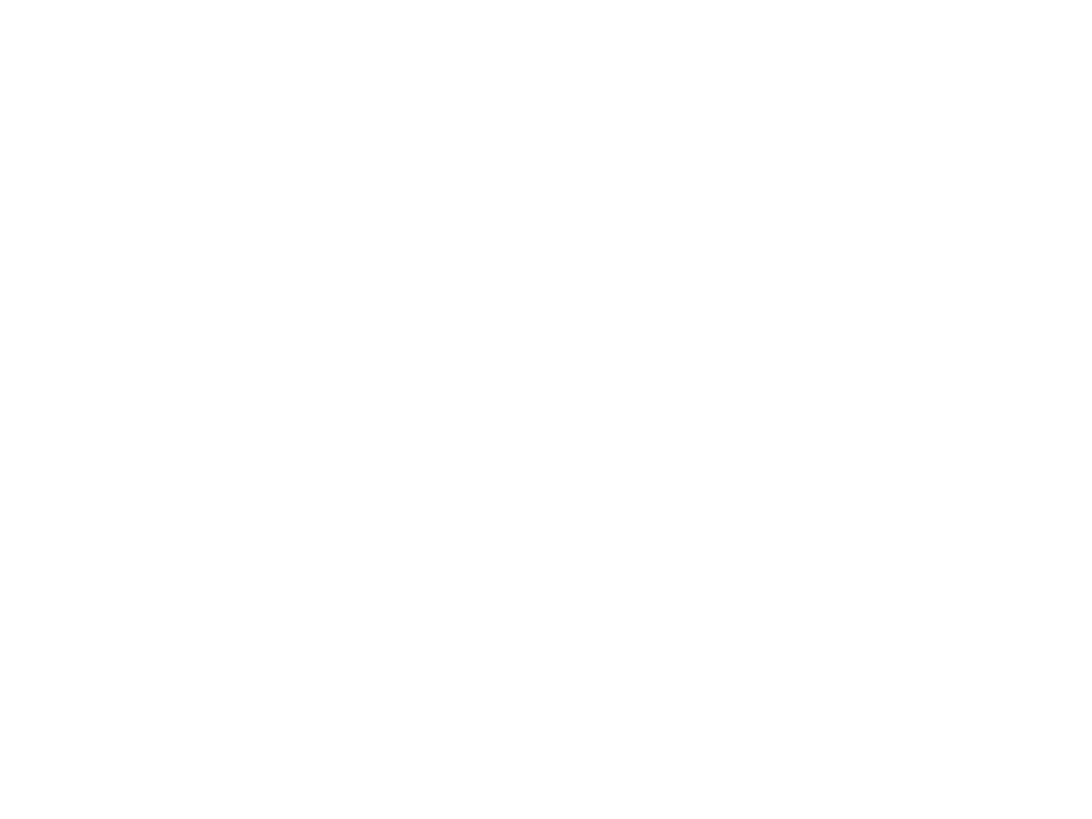
\includegraphics[width=2.5in,draft]{temp}
		\caption{Example figure Caption}
		\label{myfig}
	\end{figure}
	
	Equation (\ref{IA_TF}) describes the ...
	
	\begin{equation}
		V_{out} = \frac{R_3}{R_2}\left(1+2\frac{R_1}{R_G}\right)(V_{e1}-V_{e2})+V_g
		\label{IA_TF}
	\end{equation}
	
	\newpage % force pagebreaks where needed
	
	\subsection{Example Subsections}
	
	\section{Conclusion} %Remember: Self Contained strong conclusion
	
	While...
	
	% References Section
	\clearpage
	\IEEEtriggeratref{4} %Set to even out columns
	\nocite{*} %Remember to remove and check before submiting
	\bibliographystyle{IEEEtran}
	\bibliography{bibliography}
\end{document}


% Common Templates
\begin{comment}
	
	\begin{figure}[!t]
		\centering
		\includegraphics[width=2.5in]{myfigure}
		\caption{Simulation results for the network.}
		\label{fig_sim}
	\end{figure}
	
	\begin{figure*}[!t]
		\centering
		\subfloat[Case I]{\includegraphics[width=2.5in]{box}%
			\label{fig_first_case}}
		\hfil
		\subfloat[Case II]{\includegraphics[width=2.5in]{box}%
			\label{fig_second_case}}
		\caption{Simulation results for the network.}
		\label{fig_sim}
	\end{figure*}
	
	\begin{table}[!t]
		\renewcommand{\arraystretch}{1.3}
		\caption{An Example of a Table}
		\label{table_example}
		\centering
		\begin{tabular}{|c||c|}
			\hline
			One & Two\\
			\hline
			Three & Four\\
			\hline
		\end{tabular}
	\end{table}
	
	% When number of authors goes beyond 4 use this alternative format:
	\author{\IEEEauthorblockN{Michael Shell\IEEEauthorrefmark{1},Homer Simpson\IEEEauthorrefmark{2},James Kirk\IEEEauthorrefmark{3}, Montgomery Scott\IEEEauthorrefmark{3} and Eldon Tyrell\IEEEauthorrefmark{4}}
		\IEEEauthorblockA{\IEEEauthorrefmark{1}School of Electrical and Computer Engineering\\Georgia Institute of Technology,Atlanta, Georgia 30332--0250\\ Email: see http://www.michaelshell.org/contact.html}
		\IEEEauthorblockA{\IEEEauthorrefmark{2}Twentieth Century Fox, Springfield, USA\\Email: homer@thesimpsons.com}
		\IEEEauthorblockA{\IEEEauthorrefmark{3}Starfleet Academy, San Francisco, California 96678-2391\\Telephone: (800) 555--1212, Fax: (888) 555--1212}
		\IEEEauthorblockA{\IEEEauthorrefmark{4}Tyrell Inc., 123 Replicant Street, Los Angeles, California 90210--4321}}
	
	% Manual Bibliography Entries
	\begin{thebibliography}{1}
		\bibitem{IEEEhowto:kopka}
		H.~Kopka and P.~W. Daly, \emph{A Guide to \LaTeX}, 3rd~ed.\hskip 1em plus
		0.5em minus 0.4em\relax Harlow, England: Addison-Wesley, 1999.
	\end{thebibliography}
\end{comment}